\documentclass{article}
\usepackage[a4paper, margin=3cm]{geometry}
\usepackage[utf8]{inputenc}
\usepackage{amsmath}
\usepackage{amssymb}
\usepackage{verbatim}
\usepackage{dirtytalk}
\usepackage{calc}
% \usepackage{tikz}
\usepackage{pgfplots}
\usepackage{titlesec}
\usepackage{wrapfig}
\usepackage{fancyhdr}
\usepackage{xcolor}

\titleclass{\section}{top}
\newcommand\sectionbreak{\clearpage}

\fancypagestyle{plain}{
    \fancyhf{}
    \lhead{ CS4099 Notes }
    \rhead{ Georg Wölflein }
    \cfoot{ -\ \thepage\ - }
}
\pagestyle{plain}


\pgfplotsset{compat=newest}
\pgfplotsset{every axis plot post/.append style={mark=none}}
\usetikzlibrary{calc}
\usepgfplotslibrary{external, fillbetween}
\tikzexternalize[prefix=figures/]

\definecolor{darkcyan}{rgb}{0.0, 0.55, 0.55}

\title{CS4099}
\author{\vspace{-5ex}}
\date{\vspace{-5ex}}

\let\vec\mathbf
\newcommand{\norm}[1]{\left\lVert#1\right\rVert}

\pgfdeclarelayer{pre main}
\begin{document}

%\maketitle

\section{Week 2}

\paragraph{Control and output spaces}
The control space for robots is the wheels, and for neural nets the weights and biases.
The output space for robots is the movement/travel in the 2D obstacle space, and for neural nets the activation of the output layer.

\paragraph{The cost function}
Consider the output space
$$
    \vec{y} =
    \begin{bmatrix}
        y_{1} \\
        y_{2}
    \end{bmatrix}
    \in \mathbb{R}^2
.$$
The current weight configuration in the control space
$$
    \vec{w} =
    \begin{bmatrix}
        w_{1} \\
        w_{2} \\
        w_{3}
    \end{bmatrix}
    \in \mathbb{R}^3
$$
produces the initial output $\textcolor{blue}{i} \in \textbf{y}$. Our goal is $\textcolor{red}{g}  \in \textbf{y}$.




\begin{figure}[h]

    \begin{tikzpicture}

        \draw[thick, <->]
            (0, 5.5) node(y2line)[above] {$y_2$}
            |- (10, 0) node(y1line)[right] {$y_1$};

        \coordinate (i) at (2, 3);
        \coordinate (g) at (9, 3);
        \coordinate (frac_progress) at ($(i)!2cm!(g)$);
        \coordinate (frac_line_a) at (frac_progress |- y2line);
        \coordinate (frac_line_b) at (frac_progress |- y1line);

        \coordinate (dw_1) at ($(i)+(45:2cm)$);
        \coordinate (dw_2) at ($(i)+(-20:2cm)$);
        \coordinate (dw_3) at ($(i)+(-60:-2cm)$);
        \coordinate (dw_3_actual) at ($(i)+(-60:2cm)$);

        \draw[->] (i) -- (dw_1) node[above left] {$\frac{\delta \vec{y}}{\delta w_1}$};
        \draw[->] (i) -- (dw_2) node[below] {$\frac{\delta \vec{y}}{\delta w_2}$};
        \draw[->] (i) -- (dw_3) node[above] {$\frac{\delta \vec{y}}{\delta w_3}$};
        \draw[->, cyan] (i) -- (frac_progress);

        \draw[dotted, cyan] (frac_line_a) -- (frac_line_b);
        \draw[dotted] (dw_1 |- y2line) -- (dw_1 |- y1line);
        \draw[dotted] (dw_2 |- y2line) -- (dw_2 |- y1line);
        \draw[dotted] (dw_3_actual |- y2line) -- (dw_3_actual |- y1line);

        \draw[dashed] (i) -- (dw_1) -- (g);
        \draw[dashed] (i) -- (dw_2) -- (g);
        \draw[dashed] (i) -- (dw_3_actual) -- (g);
        \draw[->, dashed, cyan] (i) -- (g);

        \fill[blue] (i) circle (2pt) node[left] {$i$};
        \fill[red] (g) circle (2pt) node[right] {$g$};

    \end{tikzpicture}

    \caption{Diagram of the output space.}

\end{figure}



We define the cost function as
\begin{equation}
    C\left( \vec{w} \right) = \frac{\text{fractional progress}}{\text{total Euclidean distance}}.
\end{equation}

The \textcolor{cyan}{straight line goal-connecting path} would minimize the Euclidean distance while maximizing the fractional progress.




\section{Week 3}

\subsection{Research}
\paragraph{Simulated annealing}
This refers to a process that will temporarily accept sub-optimal (worse) values in hopes of overcoming local maxima, to reach better local minima.

\paragraph{Adam optimizer}
The name means \say{ADAptive Moment estimation}.
Instead of using a global learning rate (as in SGD), Adam \say{computes individual adaptive learning rates for different parameters from estimates of first and second moments of the gradients} \cite{adam}, i.e. the mean and variance.

\paragraph{The stripe problem in literature}
To do

\subsection{A problem that always achieves a point on the goal line (gradient of weights are at right angle)}

Consider the neural network below. Note that it does not have an activation function.

\begin{figure}[h]
    \begin{center}
        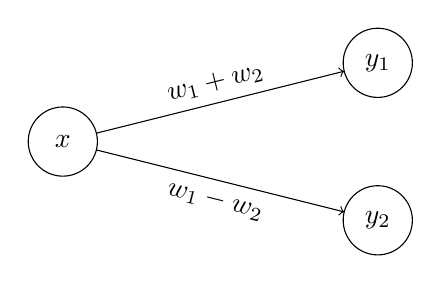
\begin{tikzpicture}
            [
                neuron/.style = {draw, circle, minimum size=25pt, inner sep=0pt, outer sep=0pt},
            ]
            
            \node [neuron] (x)  at (0,0) {$x$};
            \node [neuron] (y1) at (4,1) {$y_1$};
            \node [neuron] (y2) at (4,-1) {$y_2$};
            \draw[->] (x) -- (y1) node[midway, above, sloped] {$w_1 + w_2$};
            \draw[->] (x) -- (y2) node[midway, below, sloped] {$w_1 - w_2$};
        \end{tikzpicture}
    \end{center}
    \caption{The neural network.}
\end{figure}

Here we have
\begin{equation*}
    \vec{y}(x; \vec{w}) = 
    \begin{bmatrix}
        w_1 + w_2 \\
        w_1 - w_2
    \end{bmatrix}
    x
\end{equation*}
with the derivative
\begin{equation*}
    \frac{\partial \vec{y}}{\partial \vec{w}}
    =
    \begin{bmatrix}
        \frac{\partial y_1}{\partial w_1} & \frac{\partial y_1}{\partial w_2} \\
        \frac{\partial y_2}{\partial w_1} & \frac{\partial y_2}{\partial w_2}
    \end{bmatrix}
    =
    \begin{bmatrix}
        1 & 1 \\
        1 & -1
    \end{bmatrix}
    x.
\end{equation*}

For
$x = 1$,
let our goal be $\vec{g} = \begin{bmatrix} 10 \\ 2 \end{bmatrix}$
and the initial weight configuration be
$\vec{w} = \begin{bmatrix} 3 \\ 1 \end{bmatrix}$.
This leads to the current position $\vec{p} = \begin{bmatrix} 4 \\ 2 \end{bmatrix}$ in output space.

Say we want to achieve $\frac{1}{6}$ fractional progress, so we aim to achieve the point $\vec{q}$ at the intersection of the fractional progress line with the goal line in the diagram of Fig. \ref{fig:week3fractionlprogress}. 


\begin{figure}[h]
    \centering
    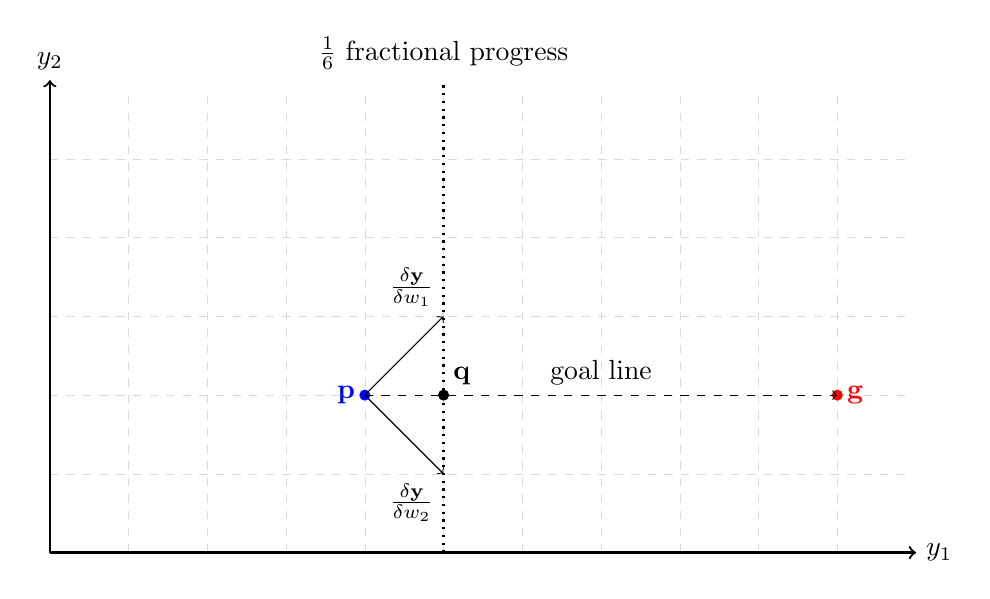
\begin{tikzpicture}
        
        \draw[help lines, color=gray!30, dashed] (0, 5.9) grid (10.9, 0);
        \draw[thick, ->] (0, 0) -- (11, 0) node[right] {$y_1$};
        \draw[thick, ->] (0, 0) -- (0, 6) node[above] {$y_2$};
        
        \coordinate (p) at (4, 2);
        \coordinate (g) at (10, 2);
        \coordinate (dw_1) at (1, 1);
        \coordinate (dw_2) at (1, -1);
        \coordinate (q) at (5, 2);
        
        \fill[blue] (p) circle (2pt) node[left] {$\vec{p}$};
        \fill[red] (g) circle (2pt) node[right] {$\vec{g}$};
        \fill (q) circle (2pt) node[above right] {$\vec{q}$};
        
        \draw[->] (p) -- +(dw_1) node[above left] {$\frac{\delta \vec{y}}{\delta w_1}$};
        \draw[->] (p) -- +(dw_2) node[below left] {$\frac{\delta \vec{y}}{\delta w_2}$};
        \draw[thick, dotted] (5, 0) -- (5, 6) node[above] {$\frac{1}{6}$ fractional progress};
        \draw[->, dashed] (p) -- (g) node[midway, above] {goal line};

    \end{tikzpicture}

    \caption{Diagram of the weights' partial derivatives in output space along with the sub-goal.}
    \label{fig:week3fractionlprogress}
\end{figure}

Now we need to find out by how much we need to update $\vec{w}$. In other words, we need to find $\vec{a} \in \mathbb{R}^2$ so that after
\begin{equation}
    \label{update_w}
    \vec{w} \leftarrow \vec{w} + \vec{a}
\end{equation}
we get
\begin{equation*}
    \vec{y}(1; \vec{w}) =
    \begin{bmatrix}
        4 \\
        2
    \end{bmatrix} + 
    \begin{bmatrix}
        1 \\
        0
    \end{bmatrix}.
\end{equation*}

This is equivalent to finding the vector $\vec{a} = \begin{bmatrix} a_1 \\ a_2 \end{bmatrix}$ that satisfies
\begin{align*}
    \begin{bmatrix}
        1 \\
        0
    \end{bmatrix}
    &=
    \frac{\partial \vec{y}}{\partial \vec{w}} \cdot \vec{a}
    \\
    &=
    a_1
    \frac{\partial \vec{y}}{\partial w_1}
    +
    a_2
    \frac{\partial \vec{y}}{\partial w_2}
    \\
    &=
    a_1
    \begin{bmatrix}
        1 \\
        1
    \end{bmatrix}
    +
    a_2
    \begin{bmatrix}
        1 \\
        -1
    \end{bmatrix},
\end{align*}
so
\begin{align*}
    a_1 = a_2 = \frac{1}{2} \\
    \vec{a} =
    \frac{1}{2}
    \begin{bmatrix}
        1 \\
        1
    \end{bmatrix}.
\end{align*}

Using (\ref{update_w}), we update $\vec{w}$ to
\begin{equation*}
    \vec{w}
    \leftarrow
    \begin{bmatrix}
        3 \\
        1
    \end{bmatrix}
    +
    \frac{1}{2}
    \begin{bmatrix}
        1 \\
        1
    \end{bmatrix}
    =
    \frac{1}{2}
    \begin{bmatrix}
        7 \\
        3
    \end{bmatrix}.
\end{equation*}


Now let's see what we get for the new $\vec{q}$ in this updated system:
\begin{equation*}
    \vec{q} =
    \vec{y}(1; \vec{w}) =
    \begin{bmatrix}
        w_1 + w_2 \\
        w_1 - w_2
    \end{bmatrix} = 
    \frac{1}{2}
    \begin{bmatrix}
        7+3 \\
        7-3
    \end{bmatrix}
    =
    \begin{bmatrix}
        5 \\
        2
    \end{bmatrix}
\end{equation*}
which is correct (see diagram).

\paragraph{Remarks:}
In this very simple example, we can use linear algebra to deterministically reach our sub-goal. 
However, as soon as we have three weights, there will be more than one possible vector $\vec{a} \in \mathbb{R}^3$ that achieves the sub-goal. 
Are there any drawbacks for choosing a particular $\vec{a}$ over another, if there are multiple options?

Furthermore, this network is so simple that the partial derivatives of the weights with respect to the output space aren't dependent on the weights themselves. However, in a \say{real} neural network, the gradients will influence each other because they depend on the weights. What happens in that case? (This question is examined in the next section.)

\subsection{When gradients are dependent on other weights}
Consider the neural network below. It uses the ReLU activation function.

\begin{figure}[h]
    \begin{center}
        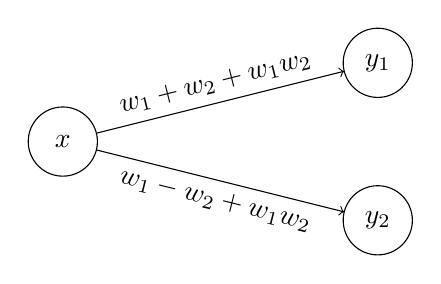
\begin{tikzpicture}
            [
                neuron/.style = {draw, circle, minimum size=25pt, inner sep=0pt, outer sep=0pt},
            ]
            
            \node [neuron] (x)  at (0,0) {$x$};
            \node [neuron] (y1) at (4,1) {$y_1$};
            \node [neuron] (y2) at (4,-1) {$y_2$};
            \draw[->] (x) -- (y1) node[midway, above, sloped] {$w_1 + w_2 + w_1 w_2$};
            \draw[->] (x) -- (y2) node[midway, below, sloped] {$w_1 - w_2 + w_1 w_2$};
        \end{tikzpicture}
    \end{center}
    \caption{The neural network.}
\end{figure}

Here we have
\begin{equation*}
    \vec{y}(x; \vec{w}) = 
    \begin{bmatrix}
        \max \left( 0, w_1 + w_2 + w_1 w_2 \right) \\
        \max \left( 0, w_1 - w_2 + w_1 w_2 \right)
    \end{bmatrix}
    x
\end{equation*}
with the derivative
\begin{equation*}
    \frac{\partial \vec{y}}{\partial \vec{w}}
    =
    \begin{bmatrix}
        \max(0, w_2 + 1) & \max(0, w_1 + 1) \\
        \max(0, w_2 + 1) & \max(0, w_1 - 1)
    \end{bmatrix}
    x.
\end{equation*}

For
$x = 1$,
let our goal be $\vec{g} = \begin{bmatrix} 9 \\ 1 \end{bmatrix}$
and the initial weight configuration be
$\vec{w} = \begin{bmatrix} 1 \\ 1 \end{bmatrix}$.
This leads to the current position $\vec{p} = \begin{bmatrix} 3 \\ 1 \end{bmatrix}$ in output space.


\begin{figure}[h]
    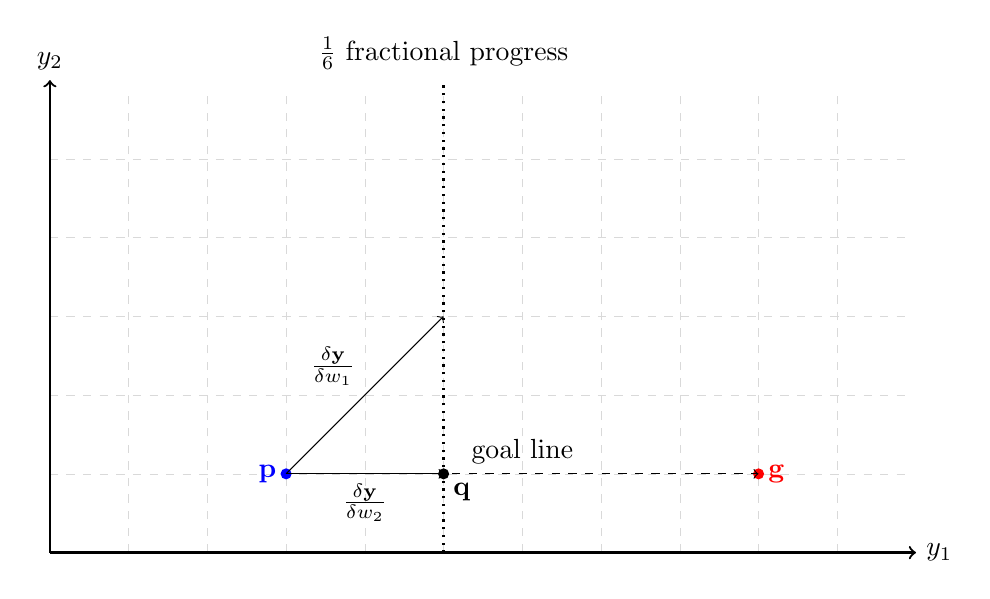
\begin{tikzpicture}
        
        \draw[help lines, color=gray!30, dashed] (0, 5.9) grid (10.9, 0);
        \draw[thick, ->] (0, 0) -- (11, 0) node[right] {$y_1$};
        \draw[thick, ->] (0, 0) -- (0, 6) node[above] {$y_2$};
        
        \coordinate (p) at (3, 1);
        \coordinate (g) at (9, 1);
        \coordinate (dw_1) at (2, 2);
        \coordinate (dw_2) at (2, 0);
        \coordinate (q) at (5, 1);
        
        \fill[blue] (p) circle (2pt) node[left] {$\vec{p}$};
        \fill[red] (g) circle (2pt) node[right] {$\vec{g}$};
        \fill (q) circle (2pt) node[below right] {$\vec{q}$};
        
        \draw[->] (p) -- +(dw_1) node[midway, above left] {$\frac{\delta \vec{y}}{\delta w_1}$};
        \draw[->] (p) -- +(dw_2) node[midway, below] {$\frac{\delta \vec{y}}{\delta w_2}$};
        \draw[thick, dotted] (5, 0) -- (5, 6) node[above] {$\frac{1}{6}$ fractional progress};
        \draw[->, dashed] (p) -- (g) node[midway, above] {goal line};

    \end{tikzpicture}

    \caption{Diagram of the weights' partial derivatives in output space along with the sub-goal.}
\end{figure}

Just looking at the diagram, one could guess to update the weights as follows to achieve $\vec{q}$:
\begin{equation*}
    \vec{w} \leftarrow \vec{w} +
    \begin{bmatrix}
        0 \\
        1
    \end{bmatrix}.
\end{equation*}
Using $\Vec{w} = \begin{bmatrix} 1 \\ 2 \end{bmatrix}$, we calculate the new output
\begin{equation*}
    \vec{y}(1; \vec{w})
    = 
    \begin{bmatrix}
        \max \left( 0, 1 + 2 + 2 \right) \\
        \max \left( 0, 1 - 2 + 2 \right)
    \end{bmatrix}
    =
    \begin{bmatrix}
        5 \\
        3
    \end{bmatrix}
\end{equation*}
which is \textit{not} our sub-goal $\vec{p}$! The reason for this is that unlike the previous network, the partial derivative $\frac{\partial \vec{y}}{\partial w_1}$ is dependent on the value of $w_2$ and vice-versa.

\paragraph{Remarks:}
When the partial derivatives are functions of each other (i.e. depend on each other), we can't use simple linear algebra in order to find the combination of the weights to achieve a specific subgoal. 
This makes intuitive sense, because if it were possible, we could simply choose the goal as our subgoal and expect to use linear algebra to find the optimum weight configuration which would eliminate the need for training neural networks.

\subsection{A problem with an unrealizable goal line, but realizable goal}
Did not find a good example yet.


\section{Week 5}

\subsection{Research}

\paragraph{Radial basis function}
A radial basis function is a real-valued function $f$ that satisfies the property $f(\vec{x}) = f(\norm{\vec{x}})$. 
RBFs are used as a kernel in SVMs. 
They are infinitely differentiable.

Two commonly used RBFs are the Gaussian function
$$ f(x) = e^{-x^2} $$
and the bump function
$$ f(x) = 
\begin{cases}
    e^{-\frac{1}{1-x^2}} & \text{for $-1<x<1$} \\
    0 & \text{otherwise}.
\end{cases}
$$

\subsection{Replicating the simple neural network with the shallow excitation gradient}
\label{sec:week5:shallownet}
Consider the very simple neural network below. 
\begin{figure}[h]
    \begin{center}
        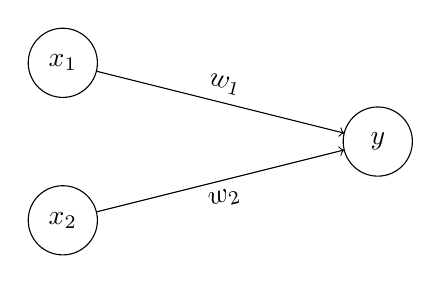
\begin{tikzpicture}
            [
                neuron/.style = {draw, circle, minimum size=25pt, inner sep=0pt, outer sep=0pt},
            ]
            
            \node [neuron] (x1)  at (0,2) {$x_1$};
            \node [neuron] (x2) at (0,0) {$x_2$};
            \node [neuron] (y) at (4,1) {$y$};
            \draw[->] (x1) -- (y) node[midway, above, sloped] {$w_1$};
            \draw[->] (x2) -- (y) node[midway, below, sloped] {$w_2$};
        \end{tikzpicture}
    \end{center}
    \caption{The neural network.}
    \label{fig:week5:shallownet}
\end{figure}

The output neuron's excitation is given by 
\begin{equation*}
    y(\vec{x}; \vec{w}, b) = \vec{w} \vec{x} + b.
\end{equation*}

Consider the two points in input space
$\vec{a} = 
\begin{bmatrix}
    0.6 \\ 0.4
\end{bmatrix}$
and
$\vec{b} = 
\begin{bmatrix}
    1 \\ 0.4
\end{bmatrix}$
with the targets $y(\vec{a}) = 0.2$ and $y(\vec{b}) = 0.8$.

The current weight configuration should be such that the hyperplane in output space of the 0.5 excitation line should be given by $x_1=0.5$.
Furthermore, the current activations should be $y(\vec{a}) = 0.51$ and $y(\vec{b}) = 0.55$ such that we get the configuration outlined in Fig. \ref{week5:initial}.
\begin{figure}[h]
    
    \centering

    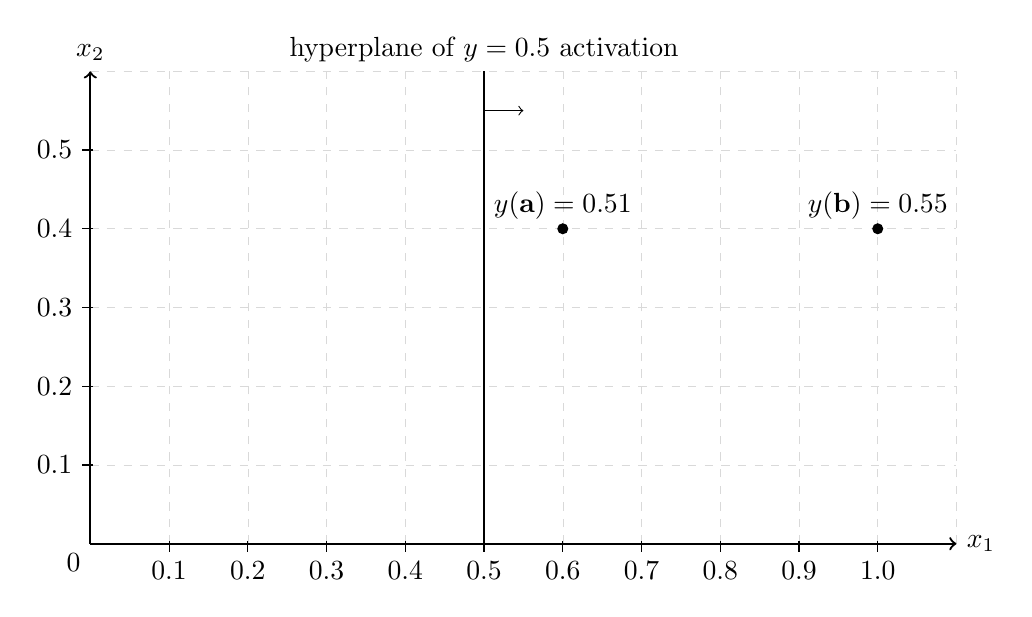
\begin{tikzpicture}[x=10cm,y=10cm]
        
        \draw[help lines, color=gray!30, dashed] (0, .6) grid (1.1, 0);
        \draw[thick, ->] (0, 0) -- (1.1, 0) node[right] {$x_1$};
        \draw[thick, ->] (0, 0) -- (0, .6) node[above] {$x_2$};
        \foreach \x in {0.1, 0.2, 0.3, 0.4, 0.5, 0.6, 0.7, 0.8, 0.9, 1.0 }
     		\draw (\x,1pt) -- (\x,-3pt)
            node[anchor=north] {\x};
        \foreach \y in {0.1, 0.2, 0.3, 0.4, 0.5 }
            \draw (1pt,\y) -- (-3pt,\y)
           node[anchor=east] {\y};
        \draw (0, 0) node[below left] {0};
        
        \draw (0.5, 0) -- (.5, .6) node[above] {hyperplane of $y=0.5$ activation};
        
        \coordinate (a) at (.6, .4);
        \coordinate (b) at (1, .4);
        
        \fill (a) circle (2pt) node[above] {$y(\vec{a})=0.51$};
        \fill (b) circle (2pt) node[above] {$y(\vec{b})=0.55$};

        \draw[->] (.5, .55) -- (.55, .55);
    \end{tikzpicture}

    \caption{The initial configuration with the hyperplane. The arrow is pointing in the direction of increasing activation.}
    \label{week5:initial}
\end{figure}

After some experimentation, it was established that this configuration can be achieved using
$\vec{w} = \begin{bmatrix}
    0.1 \\ 0.0005
\end{bmatrix}$
and $b = 0.45$ thus leading to the function
\begin{equation*}
    y(\vec{x}) = 0.1 x_1 + 0.0005 x_2 + 0.45.
\end{equation*}

\paragraph{Remarks:}
To get a gradient this shallow, it was necessary to introduce a third parameter $b$. 
We need to investigate whether we can call it a \say{non-trainable variable}, so we effectively only have two weights.

\section{Week 6}

\subsection{The hyperplanes of radial basis activation functions}
Consider the radial basis function
\begin{equation}
    \label{eq:week5:rbf}
    \phi(x) = e^{-x^2}
\end{equation}
with the graph pictured in Fig. \ref{fig:week6:rbf:plot}.

\begin{figure}[h]
    \centering
    \begin{tikzpicture}[scale=1.5]
        \draw[help lines, color=gray!30, dashed] (-3, 0) grid (3, 2);
        \draw[thick, <->] (-3.2, 0) -- (3.2, 0) node[right] {$x$};
        \draw[thick, ->] (0, 0) -- (0, 2.2) node[above] {$\phi(x)$};
        \draw[domain=-3:3,smooth,variable=\x,blue] plot ({\x},{exp(-\x*\x)});

        \foreach \x in {-3,...,3}
            \draw (\x,1pt) -- (\x,-3pt)
            node[anchor=north] {\x};
        \foreach \y in {1, ..., 2}
            \draw (1pt,\y) -- (-3pt,\y)
            node[anchor=east] {\y};
    \end{tikzpicture}
    \caption{Plot of the radial basis activation function.}
    \label{fig:week6:rbf:plot}
\end{figure}

To examine the hyperplanes corresponding to this activation function, consider the very simple neural network given in Fig. \ref{fig:week6:rbf:neuralnet}. 
\begin{figure}[h]
    \centering
    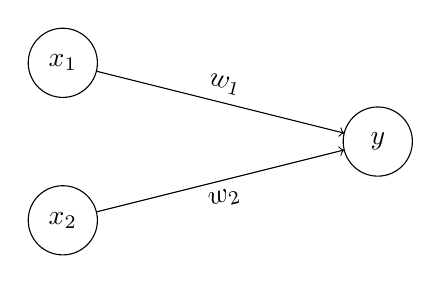
\begin{tikzpicture}
        [
            neuron/.style = {draw, circle, minimum size=25pt, inner sep=0pt, outer sep=0pt},
        ]
        
        \node [neuron] (x1)  at (0,2) {$x_1$};
        \node [neuron] (x2) at (0,0) {$x_2$};
        \node [neuron] (y) at (4,1) {$y$};
        \draw[->] (x1) -- (y) node[midway, above, sloped] {$w_1$};
        \draw[->] (x2) -- (y) node[midway, below, sloped] {$w_2$};
    \end{tikzpicture}
    \caption{The neural network.}
    \label{fig:week6:rbf:neuralnet}
\end{figure}

For simplicity, we set $w_1=w_2=1$. 
The output neuron's activation is then given by 
\begin{equation*}
    y(\vec{x}) = \phi(x_1 + x_2).
\end{equation*}

To find the equations of the hyperplanes, we set the output to 0.5, so
\begin{align*}
    \frac{1}{2} &= \phi(x_1 + x_2) \\
    &= e^{-(x_1 + x_2)^2} \\
    -\ln \frac{1}{2} &= (x_1 + x_2)^2 \\
    \pm\sqrt{-\ln \frac{1}{2}} &= x_1 + x_2 \\
    x_2 &= -x_1 \pm\sqrt{-\ln \frac{1}{2}}
\end{align*}
which means that there are two lines. They are graphed in Fig. \ref{fig:week6:rbf:hyperplanes}.

\begin{figure}[h]
    \centering
    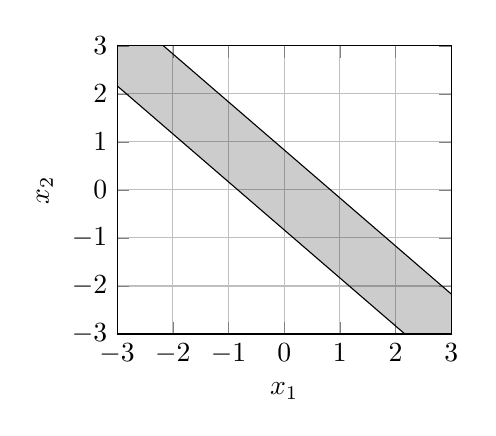
\begin{tikzpicture}
        \begin{axis}[
            scale only axis,
            width=.35\textwidth,
            % axis lines=center,
            xlabel={$x_1$},
            ylabel={$x_2$},
            ymin=-3, ymax=3,
            xmin=-3, xmax=3,
            grid,
            samples=2,
            xtick={-3,...,3},
            ytick={-3,...,3}
        ]
            \addplot[name path=A] {-x + sqrt(-ln(0.5))};
            \addplot[name path=B] {-x - sqrt(-ln(0.5))};
            \addplot[black,opacity=0.2] fill between[of=A and B];
        \end{axis}
    \end{tikzpicture}
    \hspace{.05\textwidth}
    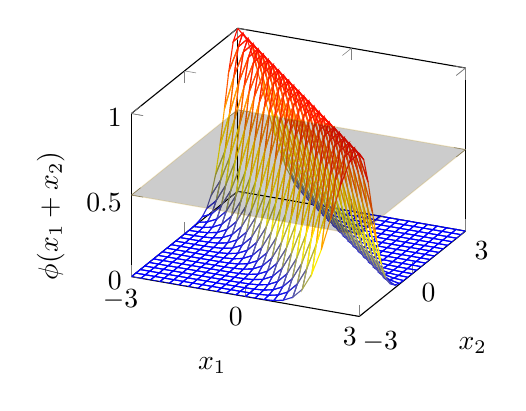
\begin{tikzpicture}
        \begin{axis}[
            scale only axis,
            width=.35\textwidth,
            ymin=-3, ymax=3,
            xmin=-3, xmax=3,
            zmin=0, zmax=1,
            xlabel={$x_1$},
            ylabel={$x_2$},
            zlabel={$\phi(x_1+x_2)$},
            samples=25,
            xtick={-3,0,3},
            ytick={-3,0,3},
            ztick={0, 1},
            extra z ticks={0.5}
        ]
            % \addplot3[
            %     name path=A,
            %     samples=2,
            %     mark=none
            % ] ({x}, {-x - sqrt(-ln(0.5))}, {0.5});
            % \addplot3[
            %     name path=B,
            %     samples=2,
            %     mark=none
            % ] ({x}, {-x + sqrt(-ln(0.5))}, {0.5});
            % \addplot3[black,opacity=0.4] fill between[of=A and B];
            \addplot3 [
                mesh,
                domain=-3:3,
                y domain=-3:3,
            ] {exp(-(x+y)^2)};
            \addplot3 [
                surf,
                fill=black,
                opacity=0.2,
                domain=-3:3,
                y domain=-3:3,
                samples=2
            ] {.5};
        \end{axis}
    \end{tikzpicture}
    \caption{Plot of hyperplanes in input space of the radial basis activation function.}
    \label{fig:week6:rbf:hyperplanes}
\end{figure}

\paragraph{Remarks:}
Notice that the radial basis function given in (\ref{eq:week5:rbf}) is differentiable and hence a suitable activation function for neural networks.
This means that if we use this activation function, we do not require hidden units in order to create a stripe configuration.

\subsection{The stripe problem without hidden units}
From the findings of the previous section, it follows that we could create the stripe problem with the neural network architecture from Fig. \ref{fig:week6:rbf:neuralnet} and the hyperplanes that are a result of the radial basis activation function.
Fig. \ref{fig:week6:rbf:hyperplanes} shows the hyperplanes for the initial weight configuration $w_1=w_2=1$.

We require four sample points to produce the problem, and they must be arranged in a way where the mean squared error is required to temporarily increase before it decreases.
The initial and possible goal configuration are shown in Fig. \ref{fig:week6:stripe:initialconfig}.

The depicted goal configuration can be achieved when either $w_1$ or $w_2$ changes to $-1$ whilst the other weight remains at $1$. In gradually changing the weight, some points will necessarily be misclassified. 

\begin{figure}[h]
    \centering
    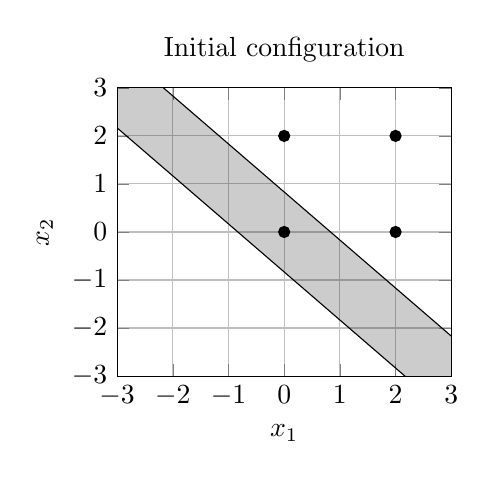
\begin{tikzpicture}
        \begin{axis}[
            scale only axis,
            width=.35\textwidth,
            title={Initial configuration},
            xlabel={$x_1$},
            ylabel={$x_2$},
            ymin=-3, ymax=3,
            xmin=-3, xmax=3,
            grid,
            samples=2,
            xtick={-3,...,3},
            ytick={-3,...,3}
        ]
            \addplot[name path=A] {-x + sqrt(-ln(0.5))};
            \addplot[name path=B] {-x - sqrt(-ln(0.5))};
            \addplot[black,opacity=0.2] fill between[of=A and B];

            \addplot [only marks] table {
                0 0
                2 2
            };
            \addplot [only marks, mark=o] table {
                0 2
                2 0
            };
        \end{axis}
    \end{tikzpicture}
    \vspace{.05\textwidth}
    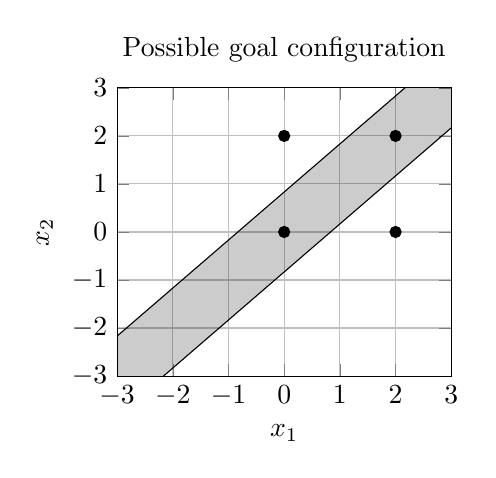
\begin{tikzpicture}
        \begin{axis}[
            scale only axis,
            width=.35\textwidth,
            title={Possible goal configuration},
            xlabel={$x_1$},
            ylabel={$x_2$},
            ymin=-3, ymax=3,
            xmin=-3, xmax=3,
            grid,
            samples=2,
            xtick={-3,...,3},
            ytick={-3,...,3}
        ]
            \addplot[name path=A] {x + sqrt(-ln(0.5))};
            \addplot[name path=B] {x - sqrt(-ln(0.5))};
            \addplot[black,opacity=0.2] fill between[of=A and B];

            \addplot [only marks] table {
                0 0
                2 2
            };
            \addplot [only marks, mark=o] table {
                0 2
                2 0
            };
        \end{axis}
    \end{tikzpicture}
    \caption{Initial and possible goal configuration for the stripe problem.}
    \label{fig:week6:stripe:initialconfig}
\end{figure}

This becomes evident when graphing the error-weight surface, as shown in Fig. \ref{fig:week6:stripe:errorsurface}. 
There is no path from the initial configuration to the global minimum with a strictly decreasing error; the error must temporarily be increased (by overcoming a hill) until reaching the global minimum trough.

\begin{figure}[h]
    \centering
    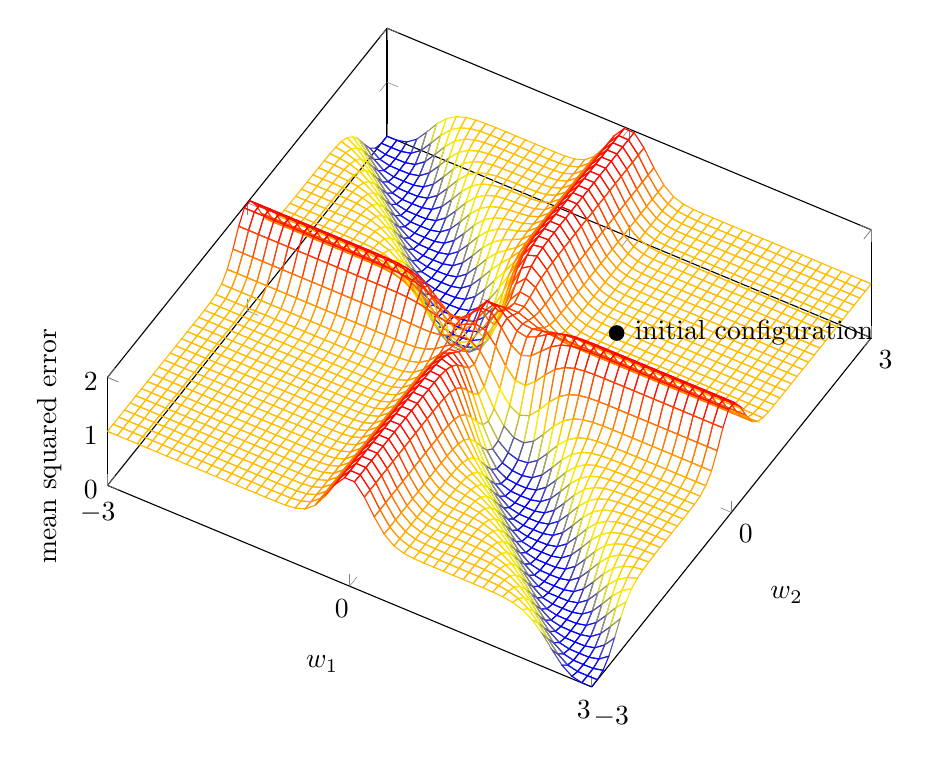
\begin{tikzpicture}
        \begin{axis}[
            scale only axis,
            width=.8\textwidth,
            ymin=-3, ymax=3,
            xmin=-3, xmax=3,
            zmin=0, zmax=2,
            xlabel={$w_1$},
            ylabel={$w_2$},
            zlabel={mean squared error},
            samples=50,
            xtick={-3,0,3},
            ytick={-3,0,3},
            ztick={0, 1, 2},
            view={30}{75}
        ]
            \addplot3 [
                mesh,
                domain=-3:3,
                y domain=-3:3
            ] {(exp(-4*x^2))^2 + (exp(-4*y^2))^2 + (1 - exp(-(2*x + 2*y)^2))^2};
            \node[label={360:{initial configuration}},circle,fill,inner sep=2pt] at (1, 1, 1) {};
        \end{axis}
    \end{tikzpicture}
    \caption{The error-weight surface of the stripe problem.}
    \label{fig:week6:stripe:errorsurface}
\end{figure}

\begin{wrapfigure}{R}{0.55\textwidth}
    \begin{tikzpicture}
        \begin{axis}[
            scale only axis,
            width = 0.4\textwidth,
            title = {Training progress},
            xlabel = {training step},
            ylabel = {loss},
            yticklabel style={/pgf/number format/.cd,fixed,precision=5}
            ]
            \addplot table {../data/week6_stripe_loss.dat};
        \end{axis}
    \end{tikzpicture}
    \caption{Loss over time during training.}
    \label{fig:week6:stripe:trainingloss}
\end{wrapfigure}

\paragraph{Training using gradient descent}
To test the above findings, this simple neural network was trained using the \texttt{keras} framework. 
As expected, the Stochastic Gradient Descent (SGD) optimizer did not achieve any noticable progress.
After 20,000 iterations, the weights were at $w_1=w_2=1.105$, i.e. they did not move to a configuration where $w_1=-w_2$ which would constitute the global minimum. 

Fig. \ref{fig:week6:stripe:trainingloss} depicts the training accuracy across the 20,000 iterations.
The only progress that was achieved was in the order of $10^{-3}$, and that was not in the direction of the global minimum.
Furthermore, the graph seems to converge to a value around $0.25$.

This means that we have found a simple example where SGD suffers the local minimum problem.

\clearpage
\subsection{Training the neural network with the shallow excitation gradient}

\begin{wraptable}{R}{0.55\textwidth}
    \begin{tabular}{c|c|c}
        point in input space & initial value & target value \\
        \hline
        $\vec{a} = \begin{bmatrix}
            0.6 \\ 0.4
        \end{bmatrix}$
        &  0.51 & 0.2 \\
        $\vec{b} = \begin{bmatrix}
            0.6 \\ 1.0
        \end{bmatrix}$
        &  0.55 & 0.8
    \end{tabular}
    \caption{Initial and target values for $\vec{a}$ and $\vec{b}$.}
    \label{table:week6:shallownet:aandb}
\end{wraptable}
Let's come back to the neural network from Sec. \ref{sec:week5:shallownet} given in Fig. \ref{fig:week5:shallownet}.
Recall the two points in input space $\vec{a}$ and $\vec{b}$ with initial and target values given in Table \ref{table:week6:shallownet:aandb}.

In order to test the behaviour of gradient descent, we will give point $\vec{b}$ a weighting four times higher than $\vec{a}$ by simply duplicating $\vec{b}$ four times in the training set which is then given by $\left\{ \vec{a}, \vec{b}, \vec{b}, \vec{b}, \vec{b}\right\}$.

The neural network was trained for 5,000 steps using \texttt{keras} and without an activation function.
Fig. \ref{fig:week6:shallownet:trainingloss} shows the training progress over time. 
It can be seen that the gradient descent optimizer initially reduces the loss quite quickly (hence the steep slope), but around step 100, the slope becomes much more shallow.
The reason for this is that until this step, the network prioritized getting a better prediction result for $\vec{b}$, but the initial rapid improvements to the four points at $\vec{b}$ caused significant deteriorations in the predictions for point $\vec{a}$.
Fig. \ref{fig:week6:shallownet:predictions} illustrates this point, as the prediction for $\vec{a}$ first moves away from the target (it increases from 0.51, instead of decreasing to the target 0.2) before performing a sharp turn around iteration 100 after which it decreased until eventually meeting 0.2.

Finally, Fig. \ref{fig:week6:shallownet:weights} shows how the weights $w_1$ and $w_2$ were updated during the training process. It can clearly be seen that SGD does not choose the optimal way of updating weights which would be a straight line from the initial weight configuration to the final configuration.

\begin{figure}[h]
    \begin{tikzpicture}
        \begin{axis}[
            scale only axis,
            width = 0.4\textwidth,
            title = {Training progress},
            xlabel = {training step},
            ylabel = {loss},
            yticklabel style={/pgf/number format/.cd,fixed},
            scaled y ticks=false,
            ymin=0, ymax=.08
            ]
            \addplot table {../data/week6_shallow_network_loss.dat};
        \end{axis}
    \end{tikzpicture}
    \vspace{.05\textwidth}
    \begin{tikzpicture}
        \begin{axis}[
            scale only axis,
            width = 0.4\textwidth,
            title = {Initial training progress (first 1,000 steps)},
            xlabel = {training step},
            ylabel = {loss},
            yticklabel style={/pgf/number format/.cd,fixed},
            scaled y ticks=false,
            ymin=0, ymax=.08, xmax=1000
            ]
            \addplot table {../data/week6_shallow_network_loss_1000.dat};
        \end{axis}
    \end{tikzpicture}
    \caption{Loss over time during training. Notice the abrupt change in gradient which can be seen in more detail on the right.}
    \label{fig:week6:shallownet:trainingloss}
\end{figure}

\begin{figure}[h]
    \begin{tikzpicture}
        \begin{axis}[
            scale only axis,
            width = 0.4\textwidth,
            title = {Predictions for $\vec{a}$ and $\vec{b}$ over time},
            xlabel = {training step},
            ylabel = {prediction ($y$)},
            legend entries = {$y(\vec{a})$, $y(\vec{b})$},
            legend style = {at={(.97,.5)}, anchor=east}
            ]
            \addplot table {../data/week6_shallow_network_predictions_a.dat};
            \addplot table {../data/week6_shallow_network_predictions_b.dat};
        \end{axis}
    \end{tikzpicture}
    \vspace{.05\textwidth}
    \begin{tikzpicture}
        \begin{axis}[
            scale only axis,
            width = 0.4\textwidth,
            title = {Predictions in relation to each other},
            xlabel = {$y(\vec{a})$},
            ylabel = {$y(\vec{b})$}
            ]
            \addplot table {../data/week6_shallow_network_predictions.dat};
        \end{axis}
    \end{tikzpicture}
    \caption{Changes in the predictions of $\vec{a}$ and $\vec{b}$ during the training process.}
    \label{fig:week6:shallownet:predictions}
\end{figure}

\begin{figure}[h]
    \begin{tikzpicture}
        \begin{axis}[
            scale only axis,
            width = 0.4\textwidth,
            title = {Changes in weights during training \\ (first 1,000 steps)},
            title style={align=center},
            xlabel = {training step},
            ylabel = {weight value},
            legend entries = {$w_1$, $w_2$},
            legend style = {at={(.97,.5)}, anchor=east}
            ]
            \addplot table {../data/week6_shallow_network_weight_0.dat};
            \addplot table {../data/week6_shallow_network_weight_1.dat};
        \end{axis}
    \end{tikzpicture}
    \vspace{.05\textwidth}
    \begin{tikzpicture}
        \begin{axis}[
            scale only axis,
            width = 0.4\textwidth,
            title = {Weights in relation to each other},
            xlabel = {$w_1$},
            ylabel = {$w_2$}
            ]
            \addplot table {../data/week6_shallow_network_weights.dat};
        \end{axis}
    \end{tikzpicture}
    \caption{Changes in weights during the training process.}
    \label{fig:week6:shallownet:weights}
\end{figure}

\bibliographystyle{apalike}
\bibliography{bibliography}

\end{document}